\chapter{Chrétiens et musulmans dans l'histoire méditerranéenne}
\mn{Charbel ATTALLAH et Marie-Carmen SMYRNELIS c.attallah@icp.fr et mc.smyrnelis@icp.fr  Chrétiens et musulmans dans l’histoire méditerranéenne : Enjeux historiques et théologiques ISTR 2022 2023 \textit{enjeux historiques et théologiques}}


\section{Introduction}

Marie Carmen Smyrnelis : Historienne de la méditerranéenne. Grecque. Villes cosmopolites du XVIII XIX

Charbel Attallah: prêtre maronite. 93 : lieu de l'islamologie. EPHE : la notion de l'amour mystique en Islam. Axe Islam et pastoral. 


\paragraph{modalité d'évaluation} fiche de lecture de Rémi Brague \textit{Y a t il eu au Moyen-âge un dialogue entre l'islam et le christianisme ?} 4 avril 4000-5000 caractères. 
Rédaction d’une fiche de lecture d’un article (4000 à 5000 caractères, espaces compris) de Rémi Brague « Y atil eu au Moyen Âge un dialogue entre l’islam et le christianisme ? » in Max Lejbowicz ( dir .), relations culturelles entre chrétiens et musulmans au Moyen Age : Quelles leçons en tirer de nos jours ?, Turnhout,  Brepols , 2005, p. 15 Les 30
\section{séances}
Double dimension du cours, théologique et historique.
Approche chronologique. 

\begin{itemize}
    \item Séance introductive islamo(à deux voix) du 17 janvier : Les enjeux du dialogue chrétien dans l’espace méditerranéen     \item Séance 2 (MarieCarmen Smyrnelis) du 24 janvier : Le statut de dhimmi de la naissance de l’islam aux Omeyyades     \item Séance 3 (Charbel dialogue islamocomme hérésie) Attallah ) du 31 janvier : Approche théologique du chrétien de la naissance de l’islam aux Omeyyades (L’islam     \item Séance 4 (MarieCarmen Smyrnelis) du 7 février : Les relations relations islamo chrétiennes  dans  un monde musulman éclaté   VIII-XI \item  Séance 5 (Charbel (VIIIe Attalla). ) du 14 février : Approche théologique des Les relations relations islamo chrétiennes  dans  un monde musulman éclaté  (VIII-XI  siècles).

    \item Séance 6 (MarieCarmen Smyrnelis) du 28 février : à l’autre et l’ère missionnaire occidentale (XIIeLa construction des identités dans leur rapport XVe siècles) \item Séance 7 (Charbel XVe siècles) \item Séance 8 (MarieAttallah ) du 7 mars : Approche théologique du dialogue islamochrétien (XIIeCarmen Smyrnelis) du 21 mars : Chrétiens et musulmans dans l’Empire ottoman  \item Séance 9 (Charbel Attallah dans l’Empire ottoman \item Séance 10 islamo(Marie) du 28 mars : Approche théologique des rapports islamo Carmen Smyrnelis) du 4 avril : chrétien au XXe siècle chrétiens De la persistance des querelles au dialogue \item Séance 11 XXe siècle (Charbel ) du 11 avril: Approche théologique du dialogue islamochrétien au \item Séance conclusive  (à deux voix) du 18 avril : Quelles perspectives pour le dialogue islamo chrétien 
\end{itemize}

\section{Objet de \Med}
\paragraph{pourquoi Méditerranéen} Creuset des civilisations. Cosmopolitisme méditerranéen qui rend une porosité entre religions.

\paragraph{Méditerranéen} 1859 : définition de la Méditerranée. Ce sont les géographes français qui le définissent. 
\paragraph{Fernand Braudel} 1000 choses à la fois. Brassage, hybridation. 

\paragraph{La Méditerranée au Liban} On tourne le dos à la mer à Beyrouth, tourné vers la montagne. Les arabes ne les intéressaient pas originellement, la mer des rums, la mer damascène. La mer blanche du milieu. Cela vient de l'expression turque par opposition à la mer noire.

\paragraph{plusieurs \Med}

D'abord une mer romaine. \textit{Mare Nostrum}
313 : liberté de culte, et donc la \Med confondue avec le Christianisme. 

\paragraph{La \Med, espace unifié ou fragmenté ?} Avec l'arrivée de L'islam, fragmentation de l'espace de la \Med. \textbf{Lac musulman} : 

\begin{quote}
    «
L’avance rapide \sn{Henri Pirenne,
Mahomet et Charlemagne , Paris, PUF, coll. Quadrige, 1992, p.} et imprévue de l’Islam […] a eu pour conséquence de
séparer définitivement l’Orient de l’Occident, en mettant fin à l’unité
méditerranéenne. Des pays comme l’Afrique et l’Espagne, qui avaient
continué à participer à la communauté occidentale, gravitent
désormais dans l’orbite de Bagdad. C’est une autre religion, une autre
culture, dans tous les domaines, qui y apparaît. La Méditerranée
occidentale, devenue un \textbf{lac musulman} , cesse d’être la voie des
échanges et idées qu’elle n’avait cessé d’être jusqu’alors. »
\end{quote}


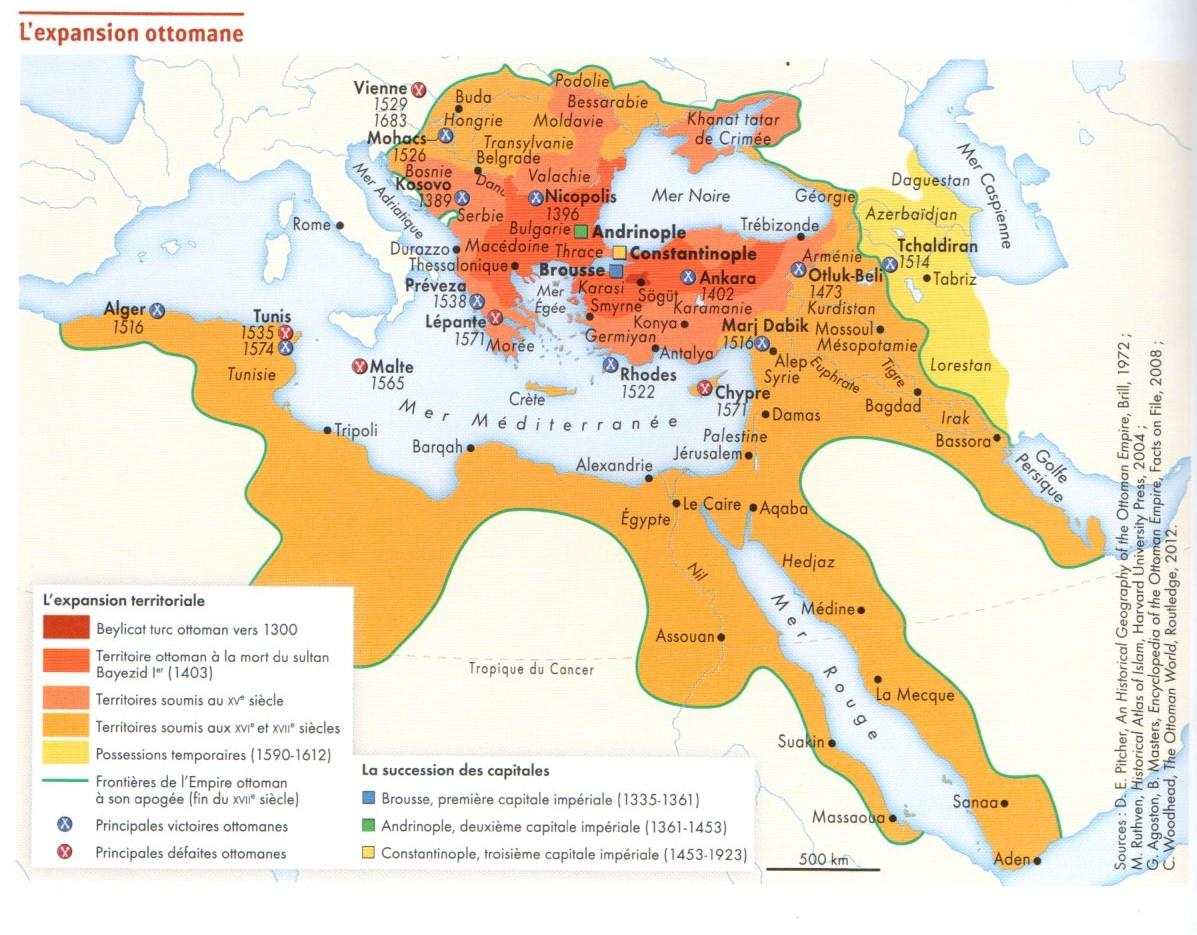
\includegraphics[width=\textwidth]{HistoireIslamMediterranee/Images/EmpireOttoman.png}
\paragraph{Fernand Braudel} s'inspire de Pirenne, mais va travailler sur l'empire des Hasbourg. Il va travailler sur la \Med dans toutes les dimensions : échange, la voir dans son unité. Il travaille avec une question : est-ce qu'il faut inventer le concept, par delà de la \Med espagnole. 

\begin{quote}
    « Dans\sn{Fernand Braudel (dir.), La Méditerranée. L’espace et l’histoire, Paris, Champs Flammarion, 1985,  p. 10} son paysage physique comme dans son paysage humain, la Méditerranée carrefour, la Méditerranée hétéroclite se présente dans nos souvenirs comme une image cohérente, comme un système où tout se mélange et se recompose dans une unité originale. Cette unité évidente, cet être profond de la Méditerranée, comment l’expliquer ? Il faudra s’y efforcer à plusieurs reprises. L’explication, ce n’est pas seulement la nature qui, à cet effet, a beaucoup œuvré ; ce n’est pas seulement l’homme, qui a tout lié ensemble obstinément ; ce sont à la fois les grâces de la nature ou ses malédictions –les unes et les autres nombreuses- et les efforts multiples des hommes, hier comme aujourd’hui. »
\end{quote}

Pour Braudel, la \Med est humaine, physique. Elle est aussi un espace d'échanges commerciaux, linguistiques. Au XIX, période la plus dense d'échanges, avec le bateau à vapeur. 


\paragraph{une \textit{rive} ou \textit{deux rives}}Après lui, les chercheurs vont s'intéresser à la définition même de l'objet : "une seule rive" : greco-romain ? ou des "deux rives", en intégrant l'héritage juif et musulman. La problématique 

\paragraph{Gardet, Berque et Massignon}{Louis Gardet, 1904-1986, philosophe chrétien des théologies comparées, islamologie. Il fonde en 1957 une revue \textit{la revue de la \Med}Il pense la \Med des deux rives, seul moyen de réduire les fractions. \textit{\Med, conception des deux rives } }. et \textit{Jacques Berque}, dépasser la rupture culturelle entre Christianisme et Islam. Islam doit fait le lien entre occident et Afrique / Asie. \textit{Louis Massignon}, Islamologue, mort en 1961, concept de l'\textit{hospitalité}. Il faut accueillir et accueillant de l'autre. Prêtre melchite en secret. Pélerinage en Côte d'Armor des 7 dormants.


\subsection{la mer partagée}

Jean Guilaine, \textit{La \Med partagée}.

La mer, qui est une mer de lien, peut être un obstacle. Avant l'Islam, des ruptures, comme en 395, la rupture entre Empire d'Orient et d'Occident. 

476 : chute de Rome.

1054 : rupture entre Eglise orient et Occident.

1204 : 4ème croisade et pillage de Constantinople.

1453 : conquête de Constantinople. 

Pirenne lui insiste sur l'irruption de l'Islam. 

D'autres insistent sur la peste du VIe siècle qui décime la \Med. 

Après les croisades, les Européens contrôlent les principales villes de la \Med mais ne connaissent pas mieux l'autre. 

\subsection{Les problématiques théologiques} 

\paragraph{Est-ce que Dieu est méditerranéen ?} Non, vue négative de la \Med. Grande mer vers le soleil couchant, mer des philistins, mer Occidentale. La fin du monde. 

\paragraph{Désert} Est-ce qu'on peut dire que le monothéisme est  méditerranéen ? Non, le monothéisme est né dans le désert. Racine sémitique, du désert, entre le Tigre et l'Euphrate.

\paragraph{Au XIIè avant JC, les phéniciens} Les maîtres de la \Med, ce sont les phéniciens qui sont sur la côte occidentale (Gaule, Carthage). La capitale de ce monde, c'est Tyr. Alphabet, art,... Est-ce une première identité mediterannéenne ? 

\paragraph{VIIème siècle : renaissance grecque archaique} \Med, plusieurs mer (Chypre, de Lybie,...). 

\paragraph{Une seule mer au temps des Romains} Avec les Romains, unité de la \Med. Paul va \textit{surfer} sur cette unité de la Mer, après la bataille d'Actium en - 31. La domination est politique mais culturellement, grecque. 

\paragraph{Une fascination de la \Med pour les Dieux} Jérusalem, Damas, 2ème capitale arabe, Rome, Constantinople + Grèce (philosophie grecque).  
\begin{quote}
   Ac 17  : Areopage 
\end{quote}
Dieu des philosophes et Dieu du désert se recontrent et ne forment plus qu'un. L'ouverture de Paul aux Nations. 

\paragraph{Conception de Jésus et la \Med.} Une ouverture à la syro-phénicienne. Jésus sort de la vision "jérusalemo-centrique".

\paragraph{Paul va s'appuyer sur l'Unité politique}
Paul. Unité religieuse de la \Med depuis 313. 3 voyages. 

\paragraph{Les fils du désert devenu des navigateurs, l'Islam} Les bébouins de l'arabie au VII vont devenir des marins. 

\paragraph{acceptation de l'Islam par la Syrie et l'Irak} 639, Syrie très vite islamisé. Pourquoi les chrétiens ont accueilli les arabes : 
\begin{itemize}
    \item peste qui a fragilisé le monde bysantin
    \item proximité culturelle
    \item un monde entre Constantinople et Perse.
    \item Nestorien
\end{itemize}

\paragraph{Apologie} de Jean Damascène 680-708. 675 : petit traité sur l'Islam. 

\paragraph{Empire Sassanide s'effondre} 
641 : l'Egypte capitule
670 : Kerouan
700 : toute l'Afrique est musulmane, plutôt paisible. 


\section{Bibliographie indicative}

\begin{itemize}
    \item     « Chrétiens et musulmans : Quel dialogue aujourd'hui ? », Cahiers de l'Atelier, tome 560, avril-juin 2019.   
    \item    ALBERA Dionigi et PENICAUD Manoël (dir.), Coexistences. Lieux saints partagés en Europe et en Méditerranée, Paris, Musée national de l’Histoire de l’Immigration – Actes sud, 2017.     
    
    \item   ALBERA Dionigi et BERTHELOT Katell (dir.) Dieu, une enquête. Judaïsme, christianisme, islam, ce qui les distingue, ce qui les rapproche, Paris, Flammarion, 2013.     
    
    \item   BERQUE Jacques, Les Arabes, Paris, Actes sud, 1999.     
    \item   BORRMANS Maurice, Prophètes du dialogue islamo-chrétien, Paris, Ed. du cerf, coll. « L’histoire à vif », 2009.     
    \item   CAHEN Claude, Islam, des origines au début de l’Empire ottoman, Paris, Hachette, coll. « Pluriel », 2011. 
    
    \item CAHEN Claude, Orient et Occident au temps des croisades, Paris, Aubier, 2010.     
    
    \item   CAILLEAUX Christophe, « Chrétiens, juifs et musulmans dans l’Espagne médiévale. La convivencia et autres mythes historiographiques », Cahiers de la Méditerranée, n°86, Juin 2013, p. 257-271.     \item   CARPENTIER Jean et LEBRUN François, Histoire de la Méditerranée, Paris, Seuil, coll. « Points Histoire », 2001.     
    \item   CAUCANAS Rémi, Relations islamo-chrétiennes en Méditerranée, entre dialogue et crispation, Presses universitaires de Rennes, 2014.   



    \item   CHEDDADI Abdesselam, Les Arabes et l'appropriation de l'histoire : émergence et premiers développements de l'historiographie musulmane jusqu'au IIe/VIIIe siècle, Paris, Actes sud, 2004.   \item DUFOURCQ Charles-Emmanuel, « La coexistence des chrétiens et des musulmans dans AlAndalus et dans le Maghrib du Xe siècle » In: Actes des congrès de la Société des historiens médiévistes de l'enseignement supérieur public, 9ᵉ congrès, Dijon, 1978, p. 209-224.  
    
    \item GAUDEUL Jean-Marie, Disputes ? Ou rencontres ?, l’islam et le christianisme au fil des siècles, Rome,   \item PISAI, coll. « Studi arabo-islamici », n°12, 1998, 2 volumes.   \item GEORGEON François, VATIN Nicolas et VEINSTEIN Gilles (dir.), Dictionnaire de l’Empire ottoman, Paris, Fayard, 2015.   \item HEYBERGER Bernard, VOGEL Jacob et ASSAN Valérie (dir.), Minorités en Méditerranée au XIXe siècle : Identités, identifications, circulations, Rennes, Presses Universitaires de Rennes, 2019.    \item HORDEN Peregrine and KINOSHITA Sharon (dir.), A Companion to Mediterranean History, Oxford, Wiley-Blackwell, 2014 (cf. Chapitre 34 “Shared Sacred Places”)    \item HOURANI Albert, Histoire des peuples arabes, Paris, Seuil, coll. « Points », 1993.   \item LEJBOWICZ Max (Eds), Les relations culturelles entre chrétiens et musulmans au Moyen Age: Quelles leçons en tirer de nos jours ?, Turnhout, Brepols, coll. « Rencontres médiévales européennes », n°5, 2005.  LOUIS Florian, Atlas historique du Moyen-Orient, Paris, Autrement, 2020.   \item MANTRAN Robert, Histoire de l’Empire ottoman, Paris, Fayard, 1989.   \item PISANI, Emmanuel,  « Le statut du ḏimmī chez al-Ġazālī », MIDÉO [En ligne], 33 | 2018, mis en ligne le 05 juillet 2018, consulté le 28 décembre 2022. URL : 
    \item REYNAERT François, La Grande Histoire du monde arabe, d'Alexandre le Grand à l'islamisme radical, Paris, Fayard, 2015.   \item REYNOLDS, Gabriel Said, The Qurʾan in Conversation with the Bible: Revised Qurʾan Translation of Ali Quli Qaraʾi annotated with Biblical Texts and Commentary by Gabriel Said Reynolds, New Haven, Yale University Press, 2018.   \item REYNOLDS, Gabriel Said, The Emergence of Islam, Minneapolis, MN Fortress Press, 2012.    \item REYNOLDS, Gabriel Said, The Qurʾān and Its Biblical Subtext, London, Routledge, 2010.   \item RODINSON Maxime, Les Arabes, Paris, PUF, coll. « Quadrige », 2002. Histoire des Arabes de 1500 à nos jours Tempus 3 ROGAN Eugene, 2016.   \item SOURDEL Dominique et Janine, 2004.   \item THOMAS History David, ROGGEMA Barbara (eds.) , Leyde  Boston, Brill, 2009 (3 volumes). , Paris, Perrin, coll. « Dictionnaire historique de l’Islam , PUF, coll. », « Quadrige », , ChristianMuslim Relations: a Bibliographical 
\end{itemize}